% Provenance (never printed): see sources/outline_sources.md (Year 2: metamorphic reactions,
% Clapeyron slopes, the Al2SiO5 diagram, the facies grid, protoliths). Definitions and facies
% table from the IUGS subcommission proposal (via the Granada translation); thermodynamic data
% from Robie and Hemingway (1995); experimental diagram from Holdaway and Mukhopadhyay (1993);
% curves from figdata/bachelor-2/facies.py; exercise and problem values in the Book 4 scratch
% calculator calc/ch10.py.
\chapter{التفاعلات التحوّلية والسحنات}\label{ch:b2:metamorphic-facies}

البازلت الذي يغوص مع صفيحته لا يبقى بازلتًا. فبلاجيوكليزه وبيروكسينه
يتفاعلان، في الحالة الصلبة، إلى معادن أخرى، وتتوقّف المجموعة الجديدة على
الضغط ودرجة الحرارة اللذين بلغهما: صخر أزرق من الغلوكوفان واللوسونيت، أو
صخر أخضر وأحمر من الأومفاسيت والغارنت. وتحتفظ الصخور المتحوّلة بهذه المعادن حين
تعود إلى السطح، وعالم الصخور الذي يعرف التفاعلات يستطيع أن يقرأ منها
الظروف. يكتب هذا الفصل تلك التفاعلات بالديناميكا الحرارية التي يدرسها
مقرّر الكيمياء، ويحسب من بيانات مقيسة أشهر مخطّط أطوار تحوّلي،
وهو مخطّط معادن \ce{Al2SiO5} الثلاثة، ويقارنه بالتجربة، وينظّم
مجموعات الصخور المتحوّلة في سحنات.
% ledger: scmr:facies-assemblages

\begin{recall}
\textbf{من مجلد المرحلة الثانوية}: \omterm{def:b2:metamorphic-facies:metamorphism}{التحوّل}، \omterm{def:b2:metamorphic-facies:metamorphism}{ودرجة التحوّل}، والمعادن الدليلية
وخطوط تساوي الدرجة، \omterm{def:b2:metamorphic-facies:metamorphism}{والتحوّل} التماسي وهالته، والتورّق والشستية،
والضغط الصخري؛ والكيانيت والأندالوسيت والسيليمانيت بوصفها متعدّدات أشكال، ومخطّط
أطوارها. \textbf{من مجلدي السنة الأولى من كتب الفيزياء والكيمياء}: طاقة
جيبس $G = H - TS$، التي تحدّد قيمتها الدنيا الحالة المستقرة عند $T$ و$P$ معلومين؛
والإنثالبي والإنتروبيا والسعة الحرارية؛ و$\mathrm dG = V\,\mathrm dP - S\,\mathrm dT$؛
وعلاقة كلاوزيوس--كلابيرون لتبخّر مادة نقية والنقطة
الثلاثية للماء. \textbf{من مجلد السنة الأولى}: نطاقات الاندساس، وأحزمة التصادم،
والتدرّج الحراري الأرضي.
\end{recall}

\section{التحوّل}\label{sec:b2:metamorphic-facies:metamorphism}

تناول مجلد المرحلة الثانوية \omterm{def:b2:metamorphic-facies:metamorphism}{التحوّل} بوصفه تحويل صخر بالحرارة
والضغط. وتعطي توصية دولية التعريف المستعمل هنا.

\begin{definition}[التحوّل؛ الصخر الأصلي]\label{def:b2:metamorphic-facies:metamorphism}
\emph{التحوّل}\index{التحوّل} عملية تغيّر معادن صخر أو
بنيته الدقيقة، أو كليهما، في الحالة الصلبة أساسًا، إذ يتكيّف الصخر
مع ظروف فيزيائية تختلف عن تلك التي تكوّن فيها وعن تلك
السائدة عادةً على سطح الأرض وفي نطاق التصخّر. وقد يتزامن مع
\omterm{def:b2:mantle-melting:melting}{الانصهار الجزئي} وقد يغيّر التركيب الكيميائي للصخر. والصخر قبل
التحوّل هو \emph{صخره الأصلي}\index{الصخر الأصلي} (البروتوليث).
\end{definition}
% ledger: scmr:metamorphism

الحدّ الأدنى يستبعد التصخّر، أي تغيّرات الرسوبيات وهي تُدفن
وتتصلّب، والحدّ الأعلى هو الانصهار، المدروس في \cref{ch:b2:crustal-melting}.
وعوامله هي درجة الحرارة، والضغط، والموائع التي تدور في الصخر (الماء
وثاني أكسيد الكربون قبل كل شيء)، والتشوّه. ويُصنَّف \omterm{def:b2:metamorphic-facies:metamorphism}{التحوّل} بحسب امتداده
وإطاره.
% ledger: scmr:metamorphism, scmr:types

يصيب \omterm{def:b2:metamorphic-facies:metamorphism}{التحوّل} \emph{الإقليمي} أحجامًا كبيرة من الصخور ويرافق
العمليات التكتونية الواسعة النطاق: فهو \emph{تحوّل جبلي} في الأحزمة الجبلية، حيث تثخن القشرة في
تصادم؛ وتحوّل \emph{الدفن} يصيب صخورًا مدفونة عميقًا تحت أكوام
رسوبية أو بركانية سميكة، دون تشوّه ولا نشاط صهاري، فتخلو صخوره
عادةً من الشستية؛ وتحوّل \emph{قاع المحيط} يبدّل القشرة قرب
ظهرات التباعد، حيث تدور فيها مياه البحر الساخنة تحت تدرّجات حرارية
شديدة، وتكون إعادة تبلوره عادةً غير مكتملة. أمّا \omterm{def:b2:metamorphic-facies:metamorphism}{التحوّل} \emph{المحلّي}
فله سبب محلّي: \omterm{def:b2:metamorphic-facies:metamorphism}{فالتحوّل} \emph{التماسي} يسخّن الصخور المضيفة لمتداخل؛
\omterm{def:b2:metamorphic-facies:metamorphism}{والتحوّل} \emph{الحرمائي} تحرّكه موائع ساخنة غنية بالماء؛
وتحوّل \emph{الانزلاق}، في نطاقات الصدوع والقصّ، يصغّر حجم الحبيبات
ويصنع الميلونيت والكاتاكلازيت؛ وتحوّل \emph{الارتطام}، تحت ارتطام نيزكي،
قد يصهر الصخر ويبخّره. ويُسمّى \omterm{def:b2:metamorphic-facies:metamorphism}{التحوّل} تقدّميًا ما دامت درجة الحرارة ترتفع
وتراجعيًا ما دامت تنخفض.
% ledger: scmr:types

\section{التفاعلات التحوّلية}\label{sec:b2:metamorphic-facies:reactions}

\begin{definition}[التفاعل التحوّلي؛ تفاعل فقد المتطايرات]\label{def:b2:metamorphic-facies:reaction}
\emph{التفاعل التحوّلي}\index{التفاعل التحوّلي} يحوّل مجموعة من معادن
صخر، هي المتفاعلات، إلى مجموعة أخرى، هي النواتج، في الحالة الصلبة، وقد
يشارك فيه طور مائع. و\emph{تفاعل فقد المتطايرات}\index{تفاعل فقد المتطايرات} تفاعل يحرّر مكوّنًا متطايرًا، الماء في تفاعل نزع الماء أو ثاني أكسيد
الكربون في تفاعل نزع الكربونات.
\end{definition}

ستظهر ثلاثة أنواع في هذا الفصل. فتغيّرات تعدّد الأشكال، كالكيانيت إلى
السيليمانيت أو الكالسيت إلى الأراغونيت، تحفظ الصيغة وتغيّر البنية.
وتفاعلات أخرى بين المواد الصلبة تعيد توزيع المكوّنات بين المعادن، كالألبيت
يعطي الجاديت والكوارتز:
\[
\ce{NaAlSi3O8 -> NaAlSi2O6 + SiO2}.
\]
وتفاعلات فقد المتطايرات تحرّر مائعًا، كتفكّك المسكوفيت والكوارتز
عند درجة حرارة مرتفعة:
\[
\ce{KAl3Si3O10(OH)2 + SiO2 -> KAlSi3O8 + Al2SiO5 + H2O}.
\]
% ledger: day73:ms-qz

لتفاعل بين معادن ثابتة التركيب، تغيّر طاقة جيبس هو
$\Delta_r G(T, P) = \sum G_{\text{النواتج}} - \sum G_{\text{المتفاعلات}}$؛ فتكون النواتج
مستقرة حيث $\Delta_r G < 0$، والمتفاعلات حيث $\Delta_r G > 0$، ويتعايش
الطرفان حيث $\Delta_r G = 0$.

\begin{definition}[التفاعل أحادي التغيّر]\label{def:b2:metamorphic-facies:univariant}
يكون تفاعل بين أطوار ثابتة التركيب \emph{أحادي التغيّر}\index{التفاعل أحادي التغيّر} حين يترك شرط توازنه $\Delta_r G(T, P) = 0$ متغيّرًا واحدًا
حرًّا: فالتوازن خط في مستوى الضغط--درجة الحرارة، يفصل
حقل المتفاعلات عن حقل النواتج.
\end{definition}

\begin{definition}[ميل كلابيرون]\label{def:b2:metamorphic-facies:clapeyron}
\emph{ميل كلابيرون}\index{ميل كلابيرون} لتفاعل هو الميل
$\mathrm dP/\mathrm dT$ لخط توازنه في مستوى الضغط--درجة الحرارة.
\end{definition}

\begin{proposition}[ميل كلابيرون لتفاعل]\label{prop:b2:metamorphic-facies:clapeyron}
على امتداد خط توازن تفاعل تغيّر إنتروبياه $\Delta_r S$ وتغيّر
حجمه $\Delta_r V$،
\[
\frac{\mathrm dP}{\mathrm dT} = \frac{\Delta_r S}{\Delta_r V}.
\]
\end{proposition}

\begin{proof}
لكل طور $\mathrm dG = V\,\mathrm dP - S\,\mathrm dT$، فللتفاعل
$\mathrm d(\Delta_r G) = \Delta_r V\,\mathrm dP - \Delta_r S\,\mathrm dT$. وعلى امتداد الخط
يبقى $\Delta_r G = 0$ صفرًا: $\Delta_r V\,\mathrm dP = \Delta_r S\,\mathrm dT$.
\end{proof}

هذه هي علاقة كلاوزيوس--كلابيرون في الفيزياء، مكتوبةً للمواد الصلبة. ومع
$\Delta_r S$ بوحدة \unit{J.mol^{-1}.K^{-1}} و$\Delta_r V$ بوحدة \unit{J.bar^{-1}} (و\unit{J.bar^{-1}} الواحد
يساوي \qty{10}{cm^3})، يخرج الميل بالبار لكل كلفن. ونتيجتان
تشكّلان كل مخطّط أطوار تحوّلي. فبين المواد الصلبة تكون تغيّرات الإنتروبيا والحجم
صغيرة، فقد يكون خط التفاعل شديد الانحدار أو قليله، موجبًا أو
سالبًا: وجهة درجة الحرارة المرتفعة تضمّ النواتج ذات الإنتروبيا الأعلى،
وجهة الضغط المرتفع تضمّ ذات الحجم الأصغر. وفي \omterm{def:b2:metamorphic-facies:reaction}{تفاعل فقد المتطايرات} يجلب المائع
إنتروبيا كبيرة، فتقع النواتج في جهة درجة الحرارة المرتفعة؛ وحجم
المائع، الكبير عند الضغط المنخفض والمتقلّص كلما ارتفع الضغط، يجعل الميل
صغيرًا عند الضغط المنخفض وأشدّ عند الضغط المرتفع. فينحني خط التفاعل.
وتضعه التجارب على المسكوفيت والكوارتز عند 603 و637 و\qty{662}{\celsius} عند 1
و2 و\qty{3}{kbar} من ضغط الماء: فبين 1 و\qty{2}{kbar} يصعد الخط
\qty{29}{bar} لكل كلفن، وبين 2 و3، \qty{40}{bar} (\cref{exo:b2:metamorphic-facies:9}).
% ledger: day73:ms-qz

\section{سيليكات الألومنيوم}\label{sec:b2:metamorphic-facies:al2sio5}

\begin{definition}[متعدّدات أشكال سيليكات الألومنيوم]\label{def:b2:metamorphic-facies:al2sio5}
\emph{متعدّدات أشكال سيليكات الألومنيوم}\index{متعدّدات أشكال سيليكات الألومنيوم} هي المعادن الثلاثة
ذات الصيغة \ce{Al2SiO5}: الكيانيت (ثلاثي الميل)، والأندالوسيت والسيليمانيت (كلاهما
معيني قائم).
\end{definition}
% ledger: rh95:al2sio5

وهي شائعة في الصخور الطينية المتحوّلة، التي تحمل ألومنيومها، ولأنها
تشترك في صيغة واحدة، فإن ما ينمو منها يتوقّف على الضغط ودرجة الحرارة وحدهما. ويعطي الجدول
أدناه خواصها المقيسة.

\begin{center}
\small
\begin{tabular}{@{}lrrrr@{}}
\hline
 & \mbox{\textdir TLT $\Delta_f H^\circ$ (\unit{kJ.mol^{-1}})} & \mbox{\textdir TLT $S^\circ$ (\unit{J.mol^{-1}.K^{-1}})} & \mbox{\textdir TLT $V^\circ$ (\unit{J.bar^{-1}})} & الكثافة \babelsublr{(\unit{g.cm^{-3}})}\\
\hline
الكيانيت & $-2593.8$ & 82.80 & 4.415 & 3.670\\
الأندالوسيت & $-2589.9$ & 91.39 & 5.152 & 3.145\\
السيليمانيت & $-2586.1$ & 95.40 & 4.986 & 3.250\\
\hline
\end{tabular}
\par\smallskip{\small الكيانيت والأندالوسيت والسيليمانيت عند \qty{298.15}{K}
و\qty{1}{bar} (روبي وهمنغواي، 1995)؛ والإنثالبيات غير مؤكدة بمقدار
\qty{2.0}{kJ.mol^{-1}}، والإنتروبيات بمقدار 0.5. والكثافة من الكتلة المولية،
\qty{162.046}{g.mol^{-1}}، والحجم.}
\end{center}
% ledger: rh95:al2sio5

الكيانيت أكثفها وأقلها إنتروبيا: فهو متعدّد الشكل المستقر عند الضغط المرتفع
ودرجة الحرارة المنخفضة. والأندالوسيت، الأقل كثافة، يستقر عند الضغط المنخفض؛ والسيليمانيت،
الأعلى إنتروبيا، يستقر عند درجة الحرارة المرتفعة. ويمكن حساب خطوط توازنها.

\begin{method}[حساب خط تفاعل]\label{met:b2:metamorphic-facies:line}
(1) من الجداول، كوّن $\Delta_r H$ و$\Delta_r S$ و$\Delta_r V$ عند \qty{298.15}{K}
و\qty{1}{bar}. (2) أهمل تغيّر $\Delta_r H$ و$\Delta_r S$ مع
درجة الحرارة (السعات الحرارية للنواتج والمتفاعلات متقاربة) وتغيّر $\Delta_r V$
مع الضغط ودرجة الحرارة (المواد الصلبة لا تكاد تنضغط أو تتمدّد):
\[
\Delta_r G(T, P) \approx \Delta_r H - T\,\Delta_r S + \Delta_r V\,(P - 1).
\]
(3) اجعله صفرًا: $P = 1 + (T\,\Delta_r S - \Delta_r H)/\Delta_r V$، وهو خط مستقيم
ميله $\Delta_r S/\Delta_r V$. (4) حيث تهمّ الدقة، استبدل بالمقدارين $\Delta_r H$
و$\Delta_r S$ قيمتيهما عند درجة الحرارة $T$، من جداول $H_T - H_{298}$ و$S_T$،
وحلّ من جديد. (5) لا تحتفظ من كل خط إلا بالجزء الذي يكون فيه طوراه أكثر استقرارًا
من أيّ طور ثالث.
\end{method}

للكيانيت إلى الأندالوسيت، $\Delta_r H = \qty{3.9}{kJ}$، $\Delta_r S =
\qty{8.59}{J.K^{-1}}$ و$\Delta_r V = \qty{0.737}{J.bar^{-1}}$: عند \qty{25}{\celsius}
و\qty{1}{bar}، $\Delta_r G = 3900 - 298.15\times8.59 = \qty{+1.34}{kJ}$، فالكيانيت،
لا الأندالوسيت، هو متعدّد الشكل المستقر على سطح الأرض؛ وللكيانيت إلى السيليمانيت
$\Delta_r G = \qty{+3.94}{kJ}$ هناك. والميول هي $8.59/0.737 = \qty{11.7}{bar/K}$
للكيانيت إلى الأندالوسيت، و$12.60/0.571 = \qty{22.1}{bar/K}$ للكيانيت إلى السيليمانيت
و$4.01/(-0.166) = \qty{-24.2}{bar/K}$ للأندالوسيت إلى السيليمانيت، وهو التفاعل الوحيد من
الثلاثة الذي يكون ناتجه في درجة الحرارة المرتفعة هو الأكثف.
% ledger: rh95:al2sio5

\begin{definition}[النقطة اللامتغيّرة]\label{def:b2:metamorphic-facies:invariant}
\emph{النقطة اللامتغيّرة}\index{النقطة اللامتغيّرة} نقطة من
مستوى الضغط--درجة الحرارة تتعايش فيها ثلاثة أطوار أو أكثر من نظام في
توازن ويلتقي فيها كل خط \omterm{def:b2:metamorphic-facies:univariant}{أحادي التغيّر} بينها؛ ولا يبقى فيها متغيّر حرّ.
\end{definition}

\begin{proposition}[النقطة الثلاثية]\label{prop:b2:metamorphic-facies:triple}
الخطوط الثلاثة الكيانيت $=$ الأندالوسيت، والكيانيت $=$ السيليمانيت، والأندالوسيت $=$
السيليمانيت تلتقي في نقطة واحدة. وحولها يكون كل خط مستقرًا في جهة واحدة فقط؛
وامتداده شبه المستقر يقع في حقل متعدّد الشكل الثالث.
\end{proposition}

\begin{proof}
لأيّ $(T, P)$، $\Delta G_{\text{كيانيت}\to\text{سيليمانيت}} = \Delta G_{\text{كيانيت}\to\text{أندالوسيت}} +
\Delta G_{\text{أندالوسيت}\to\text{سيليمانيت}}$، لأن طاقتي جيبس للأندالوسيت تتلاشيان. فحيث
يتقاطع الخطّان الأولان، ينعدم حدّان من هذه الحدود، فينعدم الثالث أيضًا: فالخط الثالث
يمرّ بالتقاطع. وبعد التقاطع، على الخط الكيانيت $=$ الأندالوسيت،
مثلًا، $G_{\text{كيانيت}} = G_{\text{أندالوسيت}}$، لكن النقطة تقع في جهة السيليمانيت من
الخطّين الآخرين، فتكون $G_{\text{سيليمانيت}}$ أصغر من كليهما: فلا الكيانيت ولا الأندالوسيت
مستقر هناك، والخط شبه مستقر.
\end{proof}

مع الخواص الثابتة في الطريقة، تقع النقطة الثلاثية عند
\qty{514}{\celsius} و\qty{3.88}{kbar} (مسألة نهاية الأسبوع)؛ ومع اعتماد الجداول على درجة
الحرارة، عند \qty{536}{\celsius} و\qty{4.20}{kbar}. أمّا المخطّط
التجريبي، المبني من تجارب معكوسة، فيضعها عند $504 \pm \qty{20}{\celsius}$
و$3.75 \pm \qty{0.25}{kbar}$ (الشكل أدناه).
% ledger: rh95:al2sio5-ht, hm93:triple, hm93:table11

\begin{omfigure}
\centering
\begin{tikzpicture}
\begin{axis}[omrecord, width=0.84\linewidth, height=7.4cm,
  xmin=200, xmax=900, ymin=0, ymax=10, xlabel={\mbox{\textdir TLT $T$ (\unit{\celsius})}}, ylabel={\mbox{\textdir TLT $P$ (\unit{kbar})}},
  legend style={font=\scriptsize, at={(0.02,0.98)}, anchor=north west},
  tick label style={font=\scriptsize}, label style={font=\small}]
\addplot[very thick, blue!70!black] table[x=T_C, y=P_kbar] {figdata/out/bachelor-2-facies-stable-kyand.dat};
\addlegendentry{\foreignlanguage{arabic}{محسوب (الجداول)}}
\addplot[thick, gray, densely dashed, mark=o, mark size=1.2pt] table[x=T_C, y=P_kbar] {figdata/out/bachelor-2-facies-hm93-kyand.dat};
\addlegendentry{تجريبي}
\addplot[thick, orange!85!black, mark=square*, mark size=1.3pt] table[x=T_C, y=P_kbar] {figdata/out/bachelor-2-facies-day73.dat};
\addlegendentry{\foreignlanguage{arabic}{مسكوفيت + كوارتز}}
\addplot[very thick, blue!70!black, forget plot] table[x=T_C, y=P_kbar] {figdata/out/bachelor-2-facies-stable-kysil.dat};
\addplot[very thick, blue!70!black, forget plot] table[x=T_C, y=P_kbar] {figdata/out/bachelor-2-facies-stable-andsil.dat};
\addplot[thin, blue!70!black, dashed, forget plot] table[x=T_C, y=P_kbar] {figdata/out/bachelor-2-facies-meta-kyand.dat};
\addplot[thin, blue!70!black, dashed, forget plot] table[x=T_C, y=P_kbar] {figdata/out/bachelor-2-facies-meta-kysil.dat};
\addplot[thin, blue!70!black, dashed, forget plot] table[x=T_C, y=P_kbar] {figdata/out/bachelor-2-facies-meta-andsil.dat};
\addplot[thick, gray, densely dashed, mark=o, mark size=1.2pt, forget plot] table[x=T_C, y=P_kbar] {figdata/out/bachelor-2-facies-hm93-kysil.dat};
\addplot[thick, gray, densely dashed, mark=o, mark size=1.2pt, forget plot] table[x=T_C, y=P_kbar] {figdata/out/bachelor-2-facies-hm93-andsil.dat};
\addplot[only marks, mark=*, mark size=2pt, blue!70!black, forget plot] table[x=T_C, y=P_kbar] {figdata/out/bachelor-2-facies-triple-B.dat};
\addplot[only marks, mark=*, mark size=2pt, gray, forget plot] table[x=T_C, y=P_kbar] {figdata/out/bachelor-2-facies-hm93-triple.dat};
\node[font=\small\bfseries] at (axis cs:330,6.2) {كيانيت};
\node[font=\small\bfseries] at (axis cs:460,0.6) {أندالوسيت};
\node[font=\small\bfseries] at (axis cs:790,3.6) {سيليمانيت};
\end{axis}
\end{tikzpicture}
\par\smallskip{\small مخطّط \ce{Al2SiO5} محسوبًا من الجداول الحرارية الديناميكية التي وضعها
روبي وهمنغواي (1995) مع إنثالبي وإنتروبيا معتمدتين على درجة الحرارة (بالأزرق؛ والمتقطّع:
الامتدادات شبه المستقرة)، والمخطّط التجريبي لهولداواي وموكوبادياي (1993)
(بالرمادي، نقاطهما المجدولة). وبالبرتقالي: تفكّك المسكوفيت + الكوارتز كما قاسه
داي (1973)، وهو منحنٍ.}
\end{omfigure}
% ledger: rh95:al2sio5, rh95:al2sio5-ht, hm93:table11, hm93:triple, day73:ms-qz

خط الكيانيت--الأندالوسيت المحسوب يقع في حدود \qty{0.1}{kbar} من الخط التجريبي
بين 400 و\qty{600}{\celsius}، لكن خط الأندالوسيت--السيليمانيت يقع
أعلى مما ينبغي بمقدار \qty{0.65}{kbar} عند \qty{600}{\celsius}. وهذا الخط أهشّ
الثلاثة: فمع $\Delta_r V = \qty{-0.166}{J.bar^{-1}}$، يحرّكه خطأ قدره \qty{0.1}{kJ} في
$\Delta_r H$، أي جزء من عشرين من عدم اليقين في كل إنثالبي في الجدول، بمقدار
\qty{600}{bar}. وإنثالبيات الجداول نفسها مضبوطة لتلائم
التجارب، في حدود عدم يقينها؛ فالتجارب، لا قياس الحرارة وحده، هي التي تثبّت
المخطّط.
% ledger: rh95:al2sio5, hm93:adjusted, hm93:table11

يُظهر الشكل أدناه لماذا يكون الخط حدًّا. فعند \qty{6}{kbar} تعبر طاقتا جيبس
للأندالوسيت والسيليمانيت، مقيستين نسبةً إلى طاقة الكيانيت، الصفرَ حيث يصبح كلٌّ منهما
أكثر استقرارًا من الكيانيت؛ والفروق لا تتجاوز أبدًا بضعة كيلوجولات لكل مول،
ولهذا يحرّك خطأ صغير في إنثالبي خطًّا كل هذه المسافة.

\begin{omfigure}
\centering
\begin{tikzpicture}
\begin{axis}[omrecord, width=0.7\linewidth, height=5.4cm,
  xmin=300, xmax=900, ymin=-4, ymax=4.5, xlabel={\mbox{\textdir TLT $T$ (\unit{\celsius})}},
  ylabel={\mbox{\textdir TLT $G - G_{\text{الكيانيت}}$ (\unit{kJ.mol^{-1}})}},
  legend style={font=\scriptsize, at={(0.02,0.02)}, anchor=south west},
  tick label style={font=\scriptsize}, label style={font=\small}]
\addplot[very thick, red!75!black] table[x=T_C, y=dG_and] {figdata/out/bachelor-2-facies-dg6.dat};
\addlegendentry{أندالوسيت}
\addplot[very thick, green!45!black] table[x=T_C, y=dG_sil] {figdata/out/bachelor-2-facies-dg6.dat};
\addlegendentry{سيليمانيت}
\addplot[thin, black] coordinates {(300,0) (900,0)};
\end{axis}
\end{tikzpicture}
\par\smallskip{\small طاقتا جيبس للأندالوسيت والسيليمانيت نسبةً إلى الكيانيت عند
\qty{6}{kbar}، من الجداول نفسها. يكون الكيانيت مستقرًا ما دام المنحنيان موجبين؛
ويحلّ محلّه السيليمانيت عند \qty{624}{\celsius}. أمّا الأندالوسيت فلا يعبر الصفر إلا عند
\qty{692}{\celsius}، حيث يكون السيليمانيت أدنى بالفعل: ففوق ضغط
النقطة الثلاثية لا يكون الأندالوسيت أبدًا الأكثر استقرارًا.}
\end{omfigure}
% ledger: rh95:al2sio5, rh95:al2sio5-ht

\begin{inthelab}[عكس تفاعل]
يُحدَّد موقع خط تفاعل في المختبر بتجارب عند ضغط ودرجة حرارة ثابتين
تبدأ من خليط من المتفاعلات والنواتج. ففي جهاز
المكبس--الأسطوانة يُحفظ الخليط من يوم إلى بضعة أيام؛ ثم يُقرأ اتجاه التفاعل
من حيود الأشعة السينية، بمقارنة نسبة قمم الناتج والمتفاعل
بنسبتها في خليط البدء، ويُؤكَّد بالنموّات الزائدة على المعدن المستقر. ودراسات
أخرى تزن بلّورة مفردة من الأندالوسيت تفاعلت في مسحوق من الكيانيت أو
السيليمانيت، بميزان مجهري دقّته نحو \qty{4}{\micro g}. ويكون التوازن
\emph{معكوسًا} حين يُرصد نموّ كل طرف على جانبي الخط؛
فيقع الخط عندئذ في المجال بينهما، مرسومًا بأخطاء الجهاز،
وهي عادةً \qty{10}{\celsius} و\qty{0.5}{kbar}. ويحكم المجرّبون على مخطّط الأطوار أولًا
بمثل هذه التجارب المعكوسة، ولا يحكمون عليه بالصخور إلا ثانيًا.
\end{inthelab}
% ledger: hm93:methods

\section{المجموعات المعدنية والسحنات}\label{sec:b2:metamorphic-facies:facies}

\begin{definition}[المجموعة المعدنية]\label{def:b2:metamorphic-facies:assemblage}
\emph{المجموعة المعدنية}\index{المجموعة المعدنية} هي مجموعة المعادن التي نمت
معًا في توازن في صخر متحوّل.
\end{definition}

تتوقّف المجموعة على ظروف \omterm{def:b2:metamorphic-facies:metamorphism}{التحوّل} وعلى تركيب
الصخر. وقد رأى إسكولا، الذي أدخل مفهوم السحنة عام 1915، أن الصخور ذات
التركيب الواحد تحمل المجموعة نفسها في الظروف نفسها، وأن
مجموعات الصخور المختلفة تتغيّر معًا حين تتغيّر الظروف؛ وتحتفظ
التوصية الدولية بمفهومه.
% ledger: scmr:facies

\begin{definition}[السحنة التحوّلية؛ شبكة السحنات]\label{def:b2:metamorphic-facies:facies}
\emph{السحنة التحوّلية}\index{السحنة التحوّلية} مجموعة من \omterm{def:b2:metamorphic-facies:assemblage}{المجموعات المعدنية}
التحوّلية، تتكرّر مقترنةً في الزمان والمكان، وتُظهر علاقة منتظمة
بين التركيب المعدني والتركيب الكيميائي الكلي، بحيث تقابل السحنات المختلفة
ظروف تحوّل مختلفة، هي أساسًا درجة الحرارة والضغط.
وتُسمّى السحنات وتُعرَّف بمجموعات الصخور ذات التركيب البازلتي.
و\emph{شبكة السحنات}\index{شبكة السحنات} هي ترتيب السحنات في
مستوى الضغط--درجة الحرارة.
\end{definition}
% ledger: scmr:facies

يسرد الجدول أدناه عشر سحنات بمعادنها المميّزة في البازلت المتحوّل.

\begin{center}
\small
\begin{tabular}{@{}p{0.27\linewidth}p{0.66\linewidth}@{}}
\hline
السحنة & المعادن المميّزة لبازلت متحوّل\\
\hline
الزيوليت & زيوليتات مثل اللومونتيت والهيولانديت\\
البرينيت--البومبيليت & برينيت + بومبيليت، برينيت + أكتينوليت، بومبيليت + أكتينوليت\\
الشيست الأخضر & أكتينوليت + ألبيت + كلوريت + إبيدوت\\
الأمفيبوليت الإبيدوتي & هورنبلند + ألبيت + إبيدوت $\pm$ كلوريت\\
الأمفيبوليت & هورنبلند + بلاجيوكليز (أكثر من \qty{17}{\percent} أنورثيت)\\
الغرانوليت & كلينوبيروكسين + أورثوبيروكسين + بلاجيوكليز؛ الأوليفين غير مستقر مع البلاجيوكليز أو الغارنت\\
الشيست الأزرق & غلوكوفان + إبيدوت $\pm$ غارنت، أو غلوكوفان + لوسونيت\\
الإكلوجيت & أومفاسيت + غارنت؛ البلاجيوكليز غير مستقر\\
هورنفلس البيروكسين & كلينوبيروكسين + أورثوبيروكسين + بلاجيوكليز؛ الأوليفين مستقر مع البلاجيوكليز\\
السانيدينيت & المجموعة نفسها، مع معادن درجات الحرارة العالية جدًّا مثل البيجونيت\\
\hline
\end{tabular}
\par\smallskip{\small السحنات ومجموعاتها المميّزة في الصخور ذات التركيب
البازلتي، وفق التوصية الدولية (سحنات إسكولا الثماني، مع سحنتي
الزيوليت والبرينيت--البومبيليت المضافتين لاحقًا).}
\end{center}
% ledger: scmr:facies-assemblages, scmr:facies

تشدّد التوصية على ما لا تفعله السحنات: فهي تسجّل انتظامات بين
المجموعات، ولا تحاول تثبيت ضغط كلٍّ منها ودرجة حرارتها. وترتيبها في
مستوى الضغط--درجة الحرارة ينتج من التفاعلات بينها، ويرسمه
الشكل أدناه رسمًا تخطيطيًا. فدرجة الحرارة ترتفع من سحنة الزيوليت مرورًا
بسحنتي الشيست الأخضر والأمفيبوليت حتى سحنة الغرانوليت؛ وعند الضغط المنخفض ودرجة
الحرارة المرتفعة تقع سحنات \omterm{def:b2:magma-emplacement:aureole}{الهورنفلس} في الهالات التماسية؛ وعند الضغط المرتفع ودرجة الحرارة
المنخفضة، سحنة الشيست الأزرق؛ وعند الضغط المرتفع ودرجة الحرارة الأعلى، سحنة
الإكلوجيت. وتثبّت تفاعلات هذا الفصل أجزاءً من الحدود: فالبلاجيوكليز،
الحاضر ألبيتًا أو بلاجيوكليزًا أغنى بالكالسيوم من سحنة الشيست الأخضر حتى سحنة الغرانوليت،
لا يستقر في سحنة الإكلوجيت، إذ
يتحوّل ألبيته إلى جاديت وكوارتز (\cref{exo:b2:metamorphic-facies:8})؛ ويتحوّل الكالسيت إلى
الأراغونيت الأكثف عند الضغط المرتفع (\cref{exo:b2:metamorphic-facies:7}).
% ledger: scmr:facies, scmr:facies-assemblages

\begin{omfigure}
\centering
\begin{tikzpicture}[font=\scriptsize, x=1cm, y=1cm]
\draw[->, thick] (0,0) -- (9.4,0) node[below left] {درجة الحرارة};
\draw[->, thick] (0,0) -- (0,6.4) node[above right] {\foreignlanguage{arabic}{الضغط (العمق)}};
\fill[orange!12] (0.3,0.1) -- (1.4,0.1) -- (1.4,1.8) -- (0.3,1.8) -- cycle;
\fill[orange!20] (1.4,0.1) -- (2.7,0.1) -- (2.7,2.6) -- (1.4,2.6) -- (1.4,1.8) -- cycle;
\fill[green!14] (2.7,0.9) -- (4.4,0.9) -- (4.4,3.6) -- (2.7,3.4) -- cycle;
\fill[green!24] (4.4,0.9) -- (5.0,0.9) -- (5.0,3.7) -- (4.4,3.6) -- cycle;
\fill[teal!18] (5.0,0.9) -- (7.0,0.9) -- (7.0,4.1) -- (5.0,3.7) -- cycle;
\fill[red!14] (7.0,0.9) -- (9.0,0.9) -- (9.0,4.6) -- (7.0,4.1) -- cycle;
\fill[gray!14] (2.7,0.1) -- (9.0,0.1) -- (9.0,0.9) -- (2.7,0.9) -- cycle;
\fill[blue!16] (1.4,2.6) -- (2.7,2.6) -- (2.7,3.4) -- (4.4,3.6) -- (3.6,6.0) -- (1.4,6.0) -- cycle;
\fill[violet!14] (4.4,3.6) -- (5.0,3.7) -- (7.0,4.1) -- (9.0,4.6) -- (9.0,6.0) -- (3.6,6.0) -- cycle;
\draw[gray, densely dashed] (1.4,0.1) -- (1.4,2.6) -- (2.7,2.6) -- (2.7,0.1);
\draw[gray, densely dashed] (0.3,1.8) -- (1.4,1.8);
\draw[gray, densely dashed] (2.7,0.9) -- (9.0,0.9);
\draw[gray, densely dashed] (4.4,0.9) -- (4.4,3.6) (5.0,0.9) -- (5.0,3.7) (7.0,0.9) -- (7.0,4.1);
\draw[gray, densely dashed] (2.7,2.6) -- (2.7,3.4) -- (4.4,3.6) -- (5.0,3.7) -- (7.0,4.1) -- (9.0,4.6);
\draw[gray, densely dashed] (4.4,3.6) -- (3.6,6.0);
\node at (0.85,0.95) {الزيوليت};
\node[align=center, font=\tiny] at (2.05,1.3) {البرينيت\\--\\البومبيليت};
\node at (3.55,2.2) {الشيست الأخضر};
\node[rotate=90] at (4.7,2.3) {\tiny الأمفيبوليت الإبيدوتي};
\node at (6.0,2.5) {الأمفيبوليت};
\node at (8.0,2.7) {الغرانوليت};
\node at (5.9,0.5) {\foreignlanguage{arabic}{سحنات الهورنفلس (الهالات التماسية)}};
\node at (2.6,4.6) {الشيست الأزرق};
\node at (6.6,5.1) {الإكلوجيت};
\end{tikzpicture}
\par\smallskip{\small \omterm{def:b2:metamorphic-facies:facies}{شبكة السحنات}، تخطيطيًا: ترتيب سحنات الجدول في
مستوى الضغط--درجة الحرارة. الحدود متدرّجة ومرسومة بلا أرقام عن
قصد: فالسحنات تُعرَّف بالمجموعات، والتفاعلات التي تحدّها تتوقّف
على تركيب كل صخر.}
\end{omfigure}
% ledger: scmr:facies, scmr:facies-assemblages

\begin{omfigure}
\centering
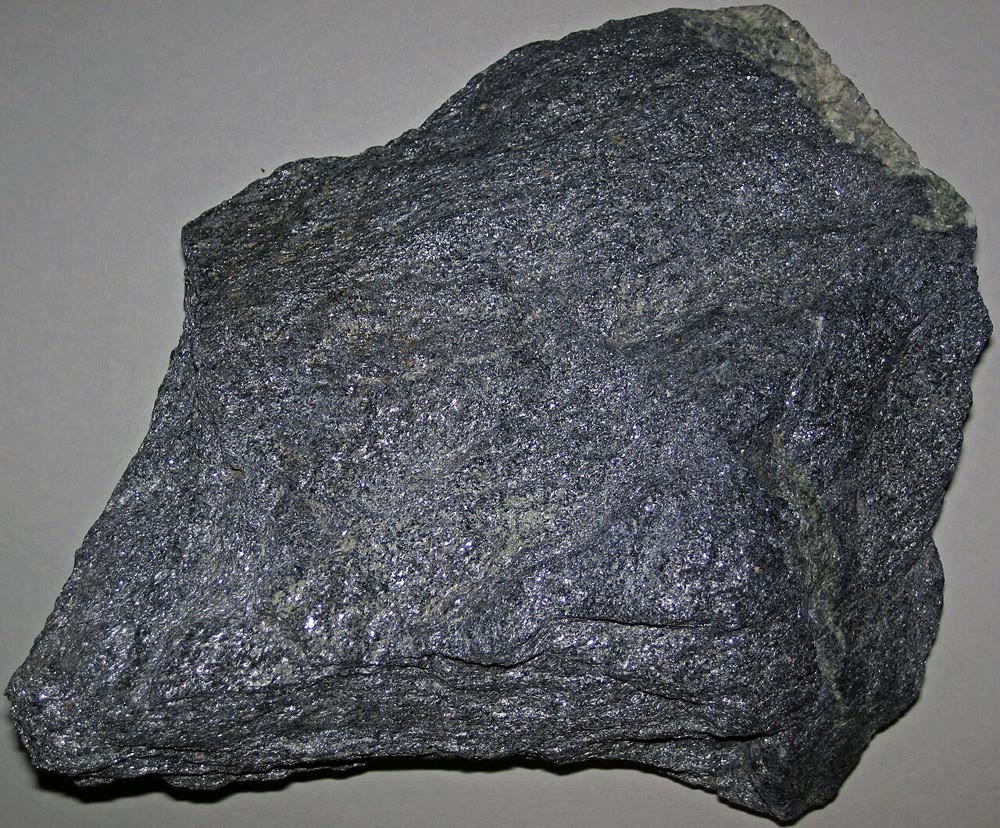
\includegraphics[width=0.27\linewidth]{images/book4/b2-10-blueschist.jpg}\hspace{0.02\linewidth}%
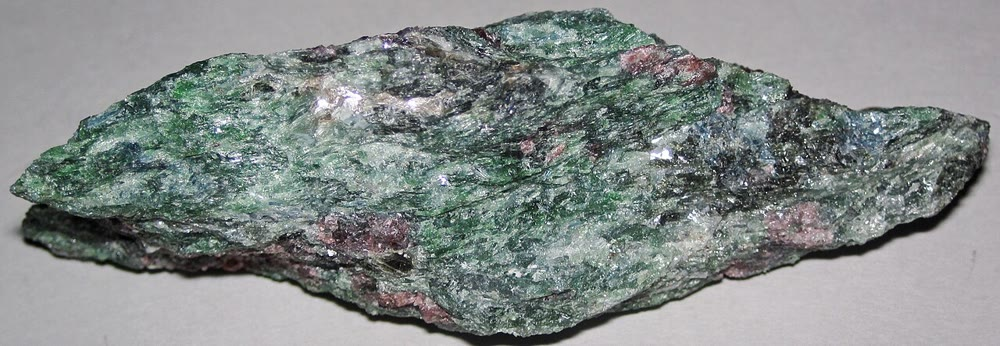
\includegraphics[width=0.69\linewidth]{images/book4/b2-10-eclogite.jpg}
\par\smallskip{\small بازلتان متحوّلان. إلى اليمين: شيست أزرق لوسونيتي من
مركّب فرانسيسكان في كاليفورنيا، أزرق بالغلوكوفان. وإلى اليسار: إكلوجيت من غرب
النرويج، أومفاسيت أخضر وغارنت أحمر مع قليل من الكوارتز والكيانيت والروتيل. الصورتان:
\mbox{\textdir TLT James St.~John, CC BY 2.0}.}
\end{omfigure}

الصخور التي تُدفن وتُسخَّن معًا تمرّ بالسحنات في ترتيب منتظم، يعكس
نسبة الضغط إلى درجة الحرارة على امتداد مسارها: مرتفعة في نطاق
اندساس، حيث تتكوّن الشيستات الزرقاء؛ ومتوسطة في حزام تصادم؛ ومنخفضة قرب متداخل.
ويسمّي \cref{ch:b2:pt-paths} هذه المتتاليات ويقرأ مثل هذه المسارات من المعادن.
% ledger: scmr:facies

\section{الصخر الأصلي مهمّ}\label{sec:b2:metamorphic-facies:protoliths}

تُعرَّف السحنات بالبازلت، لكن كل صخر أصلي يسجّل الظروف نفسها في
معادنه الخاصة.

\begin{definition}[الميتابيليت؛ الميتابازيت]\label{def:b2:metamorphic-facies:protoliths}
\emph{الميتابيليت}\index{الميتابيليت} حجر طيني متحوّل (بيليت)، غني
بالألومنيوم والبوتاسيوم، تضمّ مجموعاته الميكا والكلوريت والغارنت والستوروليت
وسيليكات الألومنيوم. و\emph{الميتابازيت}\index{الميتابازيت} بازلت متحوّل أو
غابرو أو صخر مافي آخر متحوّل، غني بالكالسيوم والمغنيسيوم والحديد، وتعرّف مجموعاته
السحنات.
\end{definition}

في \omterm{def:b2:metamorphic-facies:protoliths}{الميتابيليت} تظهر المعادن الدليلية التي عرضها مجلد المرحلة الثانوية تباعًا كلما
ارتفعت الدرجة (الكلوريت، والبيوتيت، والغارنت، والستوروليت، والكيانيت، والسيليمانيت)،
وتفاعل المسكوفيت + الكوارتز في هذا الفصل يصنع السيليمانيت والفلسبار البوتاسي عند درجة
حرارة أعلى أيضًا، وسيليكات الألومنيوم الحاضرة تخبر من أيّ جهة من النقطة
الثلاثية مرّ الصخر. والحجر الجيري أو الدولوستون المتحوّل يصير رخامًا، من الكالسيت أو
الدولوميت؛ والكربونات غير النقية، مع السيليكا والطين، تصير صخورًا كلسية سيليكاتية تحرّر
تفاعلات نزع الكربونات فيها ثاني أكسيد الكربون؛ والحجر الرملي الكوارتزي يصير كوارتزيتًا،
لا يكاد يُظهر شيئًا سوى حجم حبيباته. وميتابيليت من نطاق الكلوريت
وبازلت متحوّل بجانبه، عند الضغط ودرجة الحرارة نفسيهما، لا يتشابهان في شيء، إذ إن
الثاني صخر أخضر من الأكتينوليت والكلوريت والإبيدوت والألبيت: مجموعة واحدة من الظروف،
ومجموعتان معدنيتان.
% ledger: iugs:barrow, day73:ms-qz, scmr:facies-assemblages

\section{التمارين}

\begin{exercise}[$\star$]\label{exo:b2:metamorphic-facies:1}
سمِّ نوع \omterm{def:b2:metamorphic-facies:metamorphism}{التحوّل}: (أ) حجر جيري أُعيد تبلوره رخامًا على بُعد أقل من
\qty{500}{m} من غرانيت؛ (ب) صخر دقيق الحبيبات شريطي على امتداد صدع
انزلاقي مضربي كبير، حبيباته مسحوقة ومعاد تبلورها؛ (ج) بازلت من القشرة المحيطية تحوّل
زجاجه إلى كلوريت وزيوليتات قرب ظهرة، ولم تُستبدل معادنه إلا
جزئيًا؛ (د) أحجار رملية بركانية في قاع كومة سمكها \qty{10}{km}،
أُعيد تبلورها دون شستية.
\end{exercise}
% ledger: scmr:types

\begin{exercise}[$\star$]\label{exo:b2:metamorphic-facies:2}
من جدول سيليكات الألومنيوم، احسب $\Delta_r S$ و$\Delta_r V$
\omterm{def:b2:metamorphic-facies:clapeyron}{وميل كلابيرون} للتفاعل كيانيت $\to$ سيليمانيت، بوحدة \unit{bar/K} وبوحدة \unit{MPa/K}. وبكم
يتغيّر ضغط التوازن على مدى \qty{100}{\celsius}؟
\end{exercise}
% ledger: rh95:al2sio5

\begin{exercise}[$\star$]\label{exo:b2:metamorphic-facies:3}
إلى أيّ سحنة ينتمي كل بازلت متحوّل؟ (أ) أكتينوليت وألبيت وكلوريت
وإبيدوت؛ (ب) غلوكوفان ولوسونيت؛ (ج) هورنبلند وبلاجيوكليز فيه
\qty{30}{\percent} أنورثيت؛ (د) أومفاسيت وغارنت، دون بلاجيوكليز.
\end{exercise}
% ledger: scmr:facies-assemblages

\begin{exercise}[$\star$]\label{exo:b2:metamorphic-facies:4}
(أ) من الكتلة المولية \qty{162.046}{g.mol^{-1}} والأحجام المولية 44.15 و51.52
و\qty{49.86}{cm^3.mol^{-1}}، احسب كثافات الكيانيت والأندالوسيت والسيليمانيت.
(ب) أيّها يفضّله الضغط، ولماذا؟ (ج) تعطي قواعد بيانات المعادن 3.61 و3.15
و\qty{3.24}{g.cm^{-3}}: لماذا قد تختلف البلّورات الطبيعية عن الأطوار النقية؟
\end{exercise}
% ledger: rh95:al2sio5, webmineral:polymorphs

\begin{exercise}[$\star\star$]\label{exo:b2:metamorphic-facies:5}
للتفاعل كيانيت $\to$ أندالوسيت، $\Delta_r H = \qty{3.9}{kJ}$، $\Delta_r S =
\qty{8.59}{J.K^{-1}}$، $\Delta_r V = \qty{0.737}{J.bar^{-1}}$. (أ) أيّ متعدّد شكل
مستقر عند \qty{25}{\celsius} و\qty{1}{bar}؟ (ب) عند أيّ درجة حرارة يتعايش
الاثنان عند \qty{1}{bar}؟ (ج) احسب ضغط التوازن عند \qty{400}{\celsius}
وقارنه بالقيمة التجريبية \qty{2.54}{kbar}. (د) لماذا يوجد الأندالوسيت مع ذلك
في صخور بردت حتى السطح؟
\end{exercise}
% ledger: rh95:al2sio5, hm93:table11

\begin{exercise}[$\star\star$]\label{exo:b2:metamorphic-facies:6}
اختبر الخطوة (2) من الطريقة. عند \qty{1000}{K} تعطي الجداول المقدار $S_T$ بالقيمة 285.02 للكيانيت
و296.44 للسيليمانيت، والمقدار $(H_T - H_{298})/T$ بالقيمتين 122.29 و121.39
(\unit{J.mol^{-1}.K^{-1}}). (أ) احسب $\Delta_r H$ و$\Delta_r S$ و$\Delta_r G$ للتفاعل
كيانيت $\to$ سيليمانيت عند \qty{1000}{K} و\qty{1}{bar}. (ب) قارن بالقيم
الثابتة في الجدول. (ج) أيّ متعدّد شكل مستقر هناك، وما مقدار خطأ
الطريقة البسيطة؟
\end{exercise}
% ledger: rh95:al2sio5-ht, rh95:al2sio5

\begin{exercise}[$\star\star$]\label{exo:b2:metamorphic-facies:7}
للكالسيت والأراغونيت (\ce{CaCO3})، عند \qty{298.15}{K}، قيمتا $\Delta_f G$ هما $-1128.5$
و$-1127.4$ \unit{kJ.mol^{-1}}، وقيمتا $S$ هما 91.7 و88.0 \unit{J.mol^{-1}.K^{-1}}، وقيمتا $V$ هما 36.93
و\qty{34.15}{cm^3.mol^{-1}}، ولهما إنثالبيا تكوين متساويتان. (أ) جد
ضغط التوازن عند \qty{25}{\celsius}. (ب) احسب \omterm{def:b2:metamorphic-facies:clapeyron}{ميل كلابيرون}. (ج) جد
ضغط التوازن عند \qty{300}{\celsius}. (د) كثير من الأصداف مصنوع من الأراغونيت
ويعيش عند \qty{1}{bar}: ماذا يعني ذلك؟
\end{exercise}
% ledger: rh95:cc-ar

\begin{exercise}[$\star\star$]\label{exo:b2:metamorphic-facies:8}
للتفاعل ألبيت $\to$ جاديت + كوارتز، تعطي الجداول $\Delta_r H = \qty{-5.0}{kJ}$،
$\Delta_r S = \qty{-32.4}{J.K^{-1}}$، $\Delta_r V = \qty{-1.698}{J.bar^{-1}}$. (أ)
احسب \omterm{def:b2:metamorphic-facies:clapeyron}{ميل كلابيرون}. (ب) احسب ضغط التوازن عند \qty{500}{\celsius}.
(ج) إنثالبيات تكوين الألبيت والجاديت والكوارتز غير مؤكدة بمقدار 2.6 و3.6
و\qty{1.0}{kJ.mol^{-1}}؛ فإذا جُمعت أخطاءً مستقلة، فما مقدار عدم اليقين في ذلك
الضغط؟ (د) لماذا تخلو سحنة الإكلوجيت من البلاجيوكليز؟
\end{exercise}
% ledger: rh95:ab-jd-qz, scmr:facies-assemblages

\begin{exercise}[$\star\star$]\label{exo:b2:metamorphic-facies:9}
يتفكّك المسكوفيت + الكوارتز عند 603 و637 و\qty{662}{\celsius} تحت 1 و2
و\qty{3}{kbar}. (أ) احسب ميل الخط بين كل زوج من النقاط. (ب) إذا كانت
إنتروبيا التفاعل لا تكاد تتغيّر على هذا المدى، فبأيّ عامل تقلّص $\Delta_r V$
من المجال الأول إلى الثاني؟ (ج) أيّ طور هو المسؤول؟
\end{exercise}
% ledger: day73:ms-qz

\begin{exercise}[$\star\star\star$]\label{exo:b2:metamorphic-facies:10}
بالخواص الثابتة في الطريقة: (أ) احسب ضغوط التفاعلات الثلاثة
عند \qty{600}{\celsius}؛ (ب) بيّن أنه عند \qty{600}{\celsius} وضغط
الكيانيت $=$ الأندالوسيت، يكون السيليمانيت متعدّد الشكل الأكثر استقرارًا، فتكون هذه النقطة من
الخط شبه مستقرة؛ (ج) أيّ متعدّد شكل مستقر عند \qty{600}{\celsius}
و\qty{4}{kbar}، وعند \qty{600}{\celsius} و\qty{7}{kbar}؟
\end{exercise}
% ledger: rh95:al2sio5

\begin{exercise}[$\star\star\star$]\label{exo:b2:metamorphic-facies:11}
يحوي شيست الكيانيت والأندالوسيت والسيليمانيت معًا، وقد نمت ثلاثتها في
توازن. (أ) بالنقطة الثلاثية التجريبية، $504 \pm \qty{20}{\celsius}$
و$3.75 \pm \qty{0.25}{kbar}$، وبقشرة كثافتها \qty{2700}{kg.m^{-3}} ($g =
\qty{9.81}{m.s^{-2}}$)، على أيّ عمق نمت؟ (ب) إذا أخذنا \qty{10}{\celsius} على
السطح، فأيّ تدرّج حراري متوسط يقتضيه ذلك؟ (ج) لماذا تندر مثل هذه الصخور؟
\end{exercise}
% ledger: hm93:triple

\begin{exercise}[$\star\star\star$]\label{exo:b2:metamorphic-facies:12}
يُدفن صخران إلى العمق $z$، انطلاقًا من \qty{10}{\celsius} على السطح: الصخر X على امتداد
\qty{10}{\celsius.km^{-1}} حتى \qty{30}{km} تحت صخور كثافتها المتوسطة
\qty{3000}{kg.m^{-3}}، والصخر Y على امتداد \qty{30}{\celsius.km^{-1}} حتى \qty{20}{km} تحت صخور
كثافتها المتوسطة \qty{2800}{kg.m^{-3}}. (أ) احسب $T$ و$P$ في نهاية كل مسار.
(ب) بخطوط الخواص الثابتة (الكالسيت $=$ الأراغونيت: $P = 13.31\,T$ بار حيث $T$
بالكلفن؛ والألبيت $=$ الجاديت + الكوارتز من \cref{exo:b2:metamorphic-facies:8}؛ وسيليكات الألومنيوم من
الجدول)، أيّهما يحوي كل صخر: الأراغونيت أم الكالسيت، والجاديت + الكوارتز أم الألبيت، وأيّ
سيليكات ألومنيوم؟ (ج) أيّ المسارين هو البارد ذو الضغط المرتفع، وفي أيّ سحنة ينتهي كلٌّ منهما؟
\end{exercise}
% ledger: rh95:cc-ar, rh95:ab-jd-qz, rh95:al2sio5

\section{مسألة: بناء النقطة الثلاثية}

\begin{problem}[{مسألة نهاية الأسبوع --- مخطّط سيليكات الألومنيوم من الجداول، وإلى أيّ
حدّ يُوثق به}]
\label{pb:b2:metamorphic-facies:1}
استعمل جدول سيليكات الألومنيوم (\qty{298.15}{K}، \qty{1}{bar}) وطريقة
هذا الفصل، مع $\Delta_r H$ و$\Delta_r S$ و$\Delta_r V$ ثابتة؛ اكتب $T$ مقدّرةً بوحدة
الكلفن و$P$ بالبار، وأهمل العدد 1 في $P - 1$.

\noindent\textbf{الجزء الأول --- التفاعلات.}
\begin{enumerate}
\item احسب $\Delta_r H$ و$\Delta_r S$ و$\Delta_r V$ للتفاعل كيانيت $\to$ أندالوسيت.
\item افعل الشيء نفسه للتفاعل كيانيت $\to$ سيليمانيت.
\item افعل الشيء نفسه للتفاعل أندالوسيت $\to$ سيليمانيت، وتحقّق من أن كل خاصية هي
الفرق بين الأوليين.
\item أيّ متعدّد شكل له أكبر إنتروبيا، وأيّها له أصغر حجم؟ وفي أيّ جهة
من كل خط سيقع كلٌّ منها؟
\item احسب ميول كلابيرون الثلاثة.
\item لماذا يكون ميل التفاعل أندالوسيت $\to$ سيليمانيت سالبًا؟
\end{enumerate}

\noindent\textbf{الجزء الثاني --- أين تمرّ الخطوط.}
\begin{enumerate}[resume]
\item احسب $\Delta_r G$ للتفاعلين الأولين عند \qty{298.15}{K}. أيّ
متعدّد شكل مستقر على السطح؟
\item عند أيّ درجة حرارة (بوحدة \unit{\celsius}) يبلغ كل تفاعل التوازن عند
\qty{1}{bar}؟
\item من درجات الحرارة الثلاث في السؤال~8، أيّها توازنات مستقرة وأيّها
شبه مستقرة؟ (استعمل ترتيب الثلاث عند \qty{1}{bar}.)
\item احسب ضغط الكيانيت $=$ الأندالوسيت عند \qty{400}{\celsius}؛
وتعطي التجارب \qty{2.54}{kbar}.
\item احسب ضغط الكيانيت $=$ السيليمانيت عند \qty{700}{\celsius}؛
وتعطي التجارب \qty{7.86}{kbar}.
\item ارسم الخطوط الثلاثة تخطيطيًا بين 200 و\qty{900}{\celsius}.
\end{enumerate}

\noindent\textbf{الجزء الثالث --- النقطة الثلاثية.}
\begin{enumerate}[resume]
\item اكتب الخطين الأولين على الصورة $P = a_i T - b_i$؛ وأعطِ $a_1$ و$b_1$ و$a_2$ و$b_2$.
\item جد درجة حرارة تقاطعهما.
\item احسب ضغطه.
\item تحقّق من أن خط الأندالوسيت $=$ السيليمانيت يمرّ به.
\item قارن بالقيمتين التجريبيتين $504 \pm \qty{20}{\celsius}$ و$3.75 \pm
\qty{0.25}{kbar}$.
\item مع اعتماد الجداول على درجة الحرارة، تنتقل النقطة الثلاثية إلى
\qty{536}{\celsius} و\qty{4.20}{kbar}. هل قرّبها التحسين من
التجربة؟ وماذا يوحي ذلك عن المصدر الرئيسي للخطأ؟
\end{enumerate}

\noindent\textbf{الجزء الرابع --- إلى أيّ حدّ يُوثق به.}
\begin{enumerate}[resume]
\item ارفع إنثالبي تكوين الأندالوسيت بمقدار \qty{1}{kJ}. بكم ينتقل
خط الكيانيت $=$ الأندالوسيت في الضغط، عند درجة حرارة ثابتة؟
\item بكم تنتقل النقطة الثلاثية في درجة الحرارة؟
\item افعل الشيء نفسه لارتفاع قدره \qty{1}{kJ} في إنثالبي السيليمانيت.
\item كل إنثالبي غير مؤكدة بمقدار \qty{2.0}{kJ}. ما مدى درجات حرارة
النقطة الثلاثية الذي تسمح به بيانات قياس الحرارة وحدها؟
\item كيف إذن تستطيع الجداول الحرارية الديناميكية أن تعيد إنتاج المخطّط التجريبي في حدود
\qty{30}{\celsius}؟
\item اذكر درجة حرارة النقطة الثلاثية المحسوبة في الجزء الثالث، مقرّبةً إلى
الدرجة: الرقم الأساسي في هذه المسألة.
\end{enumerate}
\end{problem}
% ledger: rh95:al2sio5, rh95:al2sio5-ht, hm93:triple, hm93:table11, hm93:adjusted
